\section{\Large Introducción}

La propagación de ondas electromagnéticas es un aspecto fundamental en el dise\~no de redes de comunicación inalámbrica, especialmente en sistemas celulares. Los modelos de propagación permiten predecir cómo se comporta la se\~nal en diferentes condiciones ambientales, topográficas y estructurales. En esta práctica se exploran cuatro modelos fundamentales: Modelo de Espacio Libre, Superficie Reflejante, COST231-Walfish-Ikegami y Lognormal con Ensombrecimiento. Además, se aborda la detección de línea de vista (LoS), un criterio clave en la selección del modelo adecuado.

\subsection{Modelo de Espacio Libre}
Este modelo representa una condición ideal en la que no existen obstrucciones entre el transmisor y el receptor. Se basa en la ley del inverso del cuadrado y describe cómo la potencia disminuye con el cuadrado de la distancia:

\begin{equation}
L\_{fs} = 32.44 + 20\log\_{10}(d\_{km}) + 20\log\_{10}(f\_{MHz})
\end{equation}

\noindent Donde:
\begin{itemize}
\item $L\_{fs}$: Pérdida de trayectoria (dB),
\item $d\_{km}$: Distancia en kilómetros,
\item $f\_{MHz}$: Frecuencia en megahercios.
\end{itemize}

\begin{figure}[H]
\centering
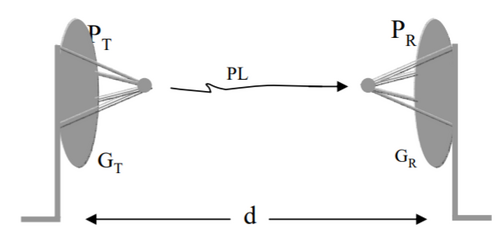
\includegraphics[width=0.5\textwidth]{./img/espaciolibre.png}
\caption{Modelo de espacio libre. La se\~nal viaja sin obstrucciones.}
\end{figure}

\subsection{Modelo de Superficie Reflejante}
Este modelo considera que la se\~nal se refleja en el suelo antes de alcanzar el receptor, generando interferencia constructiva o destructiva:

\begin{equation}
L\_{sr} = 40\log\_{10}(d\ [m]) - 20\log\_{10}(ht)(hr)
\end{equation}

\noindent Donde:
\begin{itemize}
\item $d$: Distancia en metros,
\item $ht$: Altura del transmisor,
\item $hr$: Altura del receptor.
\end{itemize}

\begin{figure}[H]
\centering
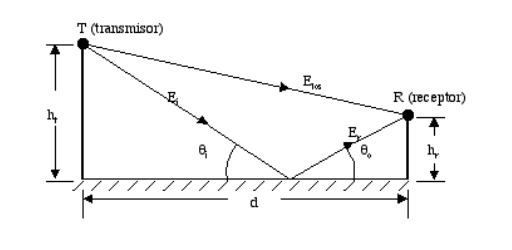
\includegraphics[width=0.5\textwidth]{./img/reflejante.png}
\caption{Modelo con reflexión en superficie terrestre.}
\end{figure}

\subsection{Modelo COST231-Walfish-Ikegami}
Este modelo se usa en entornos urbanos. Considera la influencia de edificios, calles y la geometría urbana. Se divide en pérdidas de trayectoria básica, de techo a calle y por difracción:

\begin{align}
L &= L_0 + L_{rts} + L_{msd} \\
L_0 &= 32.4 + 20\log_{10}(d_{km}) + 20\log_{10}(f_{MHz}) \\
L_{rts} &= -16.9 - 10\log_{10}(w) + 10\log_{10}(f) + 20\log_{10}(h_t - h_r) + L_{ori} \\
L_{msd} &= L_{bsh} + k_a + k_d \log_{10}(d) + k_f \log_{10}(f) - 9 \log_{10}(b)
\end{align}

\noindent Parámetros:
\begin{itemize}
\item $w$: Ancho de calle, $b$: Separación entre edificios,
\item $L_{ori}$: Pérdida por orientación, $L_{bsh}$: Pérdida techo a calle,
\item $k_a = 54$, $k_d = 18$, $k_f$: Factor de frecuencia.
\end{itemize}

\begin{figure}[H]
\centering
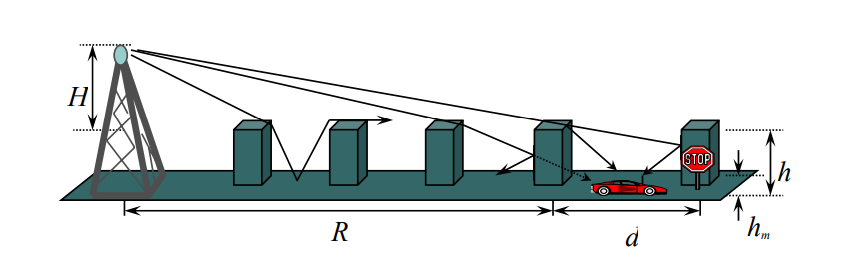
\includegraphics[width=0.5\textwidth]{./img/walfish.png}
\caption{Modelo COST231 considerando estructura urbana.}
\end{figure}

\subsection{Modelo Lognormal con ensombrecimiento}
Este modelo incorpora la variabilidad aleatoria debida a obstrucciones como edificios o árboles. La pérdida total incluye una componente aleatoria:

\begin{equation}
L\_{\log} = 10 \alpha \log\_{10}(d\_{km}) + X\_\sigma
\end{equation}

\noindent Donde:
\begin{itemize}
\item $alpha$: Exponente de pérdida,
\item $X_sigma$: Variable aleatoria normal con desviación $sigma$ (dB).
\end{itemize}

\begin{equation}
P\_{rx} = P\_{tx} + G\_{tx} + G\_{rx} - L\_{\log}
\end{equation}

\subsection{Análisis de Línea de Vista (LoS)}
La detección de LoS se basa en una evaluación geométrica entre la estación base y el receptor. Si un obstáculo (ej. edificio) intersecta la línea entre ambos puntos, se considera NLoS (Non-Line-of-Sight), lo cual modifica el modelo de propagación.

La correcta identificación de la condición LoS permite seleccionar el modelo más adecuado y obtener predicciones más precisas sobre la potencia de la se\~nal recibida.
